Figure~\ref{fig:4:fw} in Chapter~\ref{chap:cc.fw} shows the structure of the
congestion control framework described in this thesis. The framework
categorizes \emph{off-path} sources and \emph{in-band} signaling for
implementing congestion control (corresponds to \emph{Block C} in
Figure~\ref{fig:4:fw}), which are discussed in this chapter. This chapter is
based on our work on Multipath RTP (MPRTP), which is documented in
\citepub{c:mprtp}, in \cite{draft.mprtp}, \cite{draft.mprtp.sdp},
\cite{Globisch:AsymGrpComm}, and \cite{draft.rtcp.overlay}.

In \citepub{c:mprtp}, we propose design goals to implement a
multipath protocol for multimedia, protocol details, a scheduling algorithm to
send media packets over multiple paths, and a dejitter buffer implementation to
play out packets smoothly even when the path skew is high. We evaluate the
performance of the proposed mechanisms in diverse scenarios in our testbed.
Lastly, we discuss the system consideration for deployment.

In \cite{draft.mprtp}, we describe the requirements, functional blocks and
protocol formats to extend RTP for enabling multipath capabilities. However,
\cite{draft.mprtp} does not define a scheduling algorithm and therefore allows 
for multiple proposals. In \cite{draft.mprtp.sdp}, we describe SDP and RTSP extensions
required to set up MPRTP sessions and also ICE extensions to advertise MPRTP
interfaces and perform NAT traversal.

In \cite{Globisch:AsymGrpComm}, we propose using a network topology with
multiple distribution trees to distribute video streams in a very large
video conference call with few active speakers and many passive participants
listening in. The multiple distribution trees carry separate MPRTP subflows
and participants are members of multiple distribution trees, but actively
forward media flows tp one of the distribution trees. Therefore, a node is an
overlay node in a few (e.g., one) distribution trees and a leaf node in the
rest. In the paper, we use a centralized focus to manage joining, leaving
and inserting a participant in the appropriate position in the distribution
tree. \cite{draft.rtcp.overlay} is a work in progress and proposes protocol
extensions to perform tree constructions in a distribution tree without the
need for a centralized conferencing focus.


\section{Multipath RTP (MPRTP)}

The Internet backbone has evolved over the past decades into a mesh of service
providers with manifold peerings that are generally capable of offering a
number of (independent) paths between two nodes. Networks often use multiple
attachment points for resilience purposes, such as data enterprise networks or
data centers, and even routers for SOHO networks support multiple access
networks~\cite{draft.fun.multi, draft.homenet.arch}. Additionally, many hosts
today feature multiple network interfaces (e.g., WLAN and 3G on mobile
devices). This may yield the opportunity for two endpoints to communicate via
multiple paths. While exploiting multipath characteristics
\cite{Wischik:2008:RPP} has been explored for TCP (e.g.,
MPTCP~\cite{rfc6824}), the requirements for real-time traffic differs notably
and TCP can at best serve real-time communication within tight delay
constraints of the network~\cite{Brosh:tcp-real-time}. In the multipath case,
the scheduling algorithms do not consider real-time bounds when spreading data
segments across different paths, and diverse paths may lead to worst-case delay
and thus even longer buffering time.

\begin{figure}
\centerline {
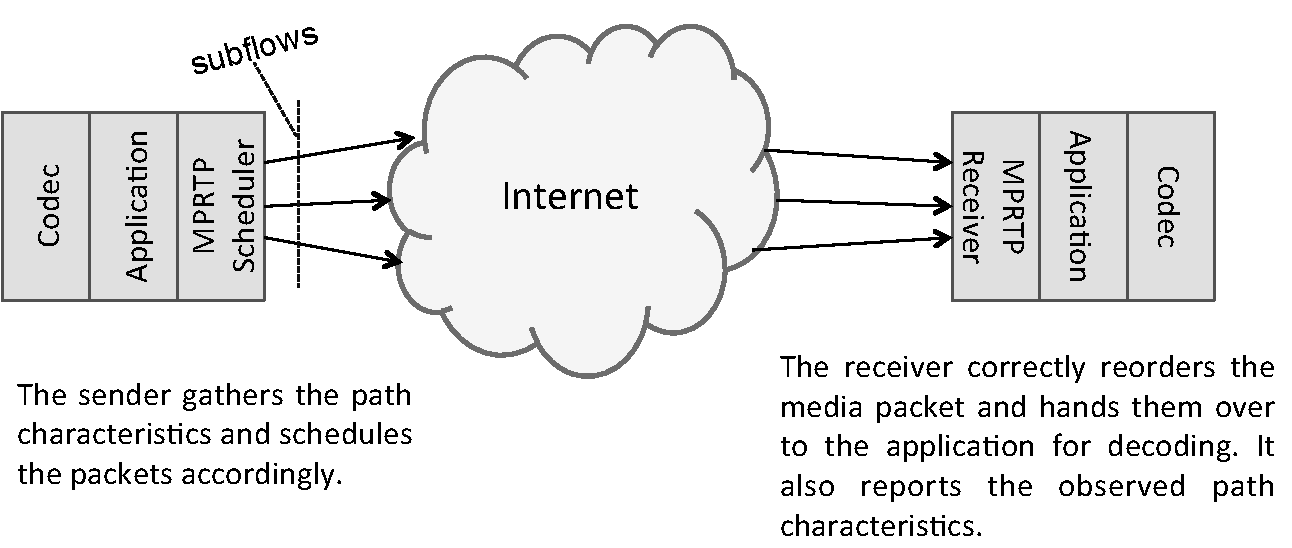
\includegraphics[width=0.9\textwidth]{chap7-fig_mprtp-1}
}
\caption{System Overview: A sender uses multiple paths to stream media
  to a receiver.  The receiver uses a dejitter buffer to reorder
  packets and sends per-path characteristics to the sender that
  distributes the packets based on the reported values.}
\label{chap7:fig_mprtp}
\end{figure}

We propose Multipath RTP (MPRTP) as a backwards-compatible extension to
RTP~\cite{rfc3550}. It is documented in \cite{draft.mprtp} and defines the
basic mechanisms to operate across multiple parallel paths.
Figure~\ref{chap7:fig_mprtp} shows a macroscopic system overview of MPRTP. The
primary use-case for MPRTP is transporting media flows between multi-homed
endpoints. Such endpoints could be residential IPTV or telepresence devices
that connect to the Internet through two different Internet service providers
(ISPs), or mobile devices that connect to the Internet through 3G and WLAN
interfaces. By allowing RTP to use multiple paths for transmission, the
following gains can be achieved:

\begin{enumerate}
\setlength{\itemsep}{5pt}

\item \textbf{\texttt{Higher quality}}: Pooling the resource capacity of
multiple Internet paths allows higher bit-rate and higher quality codecs to be
used. From the application perspective, the overall available capacity between the
two endpoints increases.

\item \textbf{\texttt{Load balancing}}: Transmitting an RTP stream over
multiple paths reduces the capacity usage on a single path, which in turn
reduces the impact of the media stream on other traffic on that path. Also,
seamlessly offloading a flow from one path to another allows for some gains
such as reduced energy consumption, reduced access costs, or reduced
network latency.

\item \textbf{\texttt{Fault tolerance}}: Using multiple paths in conjunction
with redundancy mechanisms (FEC, re-transmissions, etc.), outages on one path
have less impact on the overall perceived quality of the stream. This can also
enable seamless handover in the case of mobility, i.e., moving from one
network to another.

\end{enumerate}


\begin{figure}
\centerline {
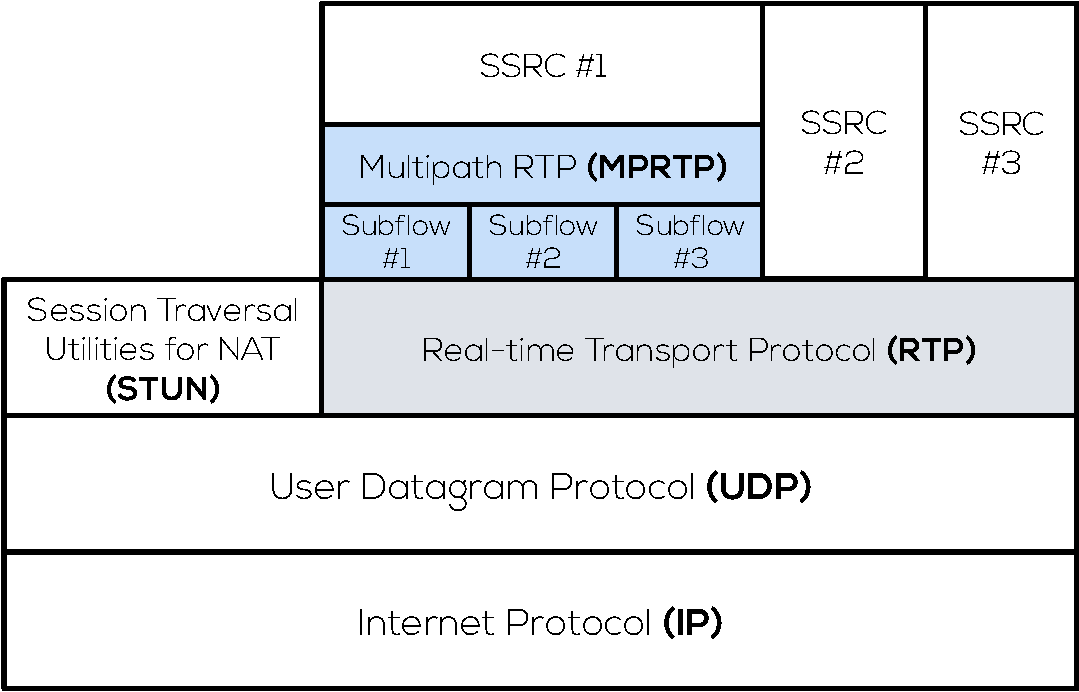
\includegraphics[width=0.75\textwidth]{chap7-fig-mprtp-stack}
}
\caption{The RTP and MPRTP stack working alongside each other. SSRC $\#1$ uses
MPRTP while SSRC $\#2$ and SSRC $\#3$ uses single path RTP.}
\label{chap7:fig_mprtp_arch}
\end{figure}

Figure~\ref{chap7:fig_mprtp_arch} compares the network stack of a single path
and a multipath-capable endpoints. SSRC \#2 and SSRC \#3 use a single path,
while SSRC \#1 uses multiple paths (with two subflows for the two interfaces).
Subflow \#1 and \#2 are expected to flow over IP address \#1 and \#2,
respectively. To discover its available interfaces, the multimedia application
either uses the ICE procedures (hence, STUN) or implements a similar
lightweight interface discovery process.

The design goals for MPRTP from our perspective are: an MPRTP-enabled system that 
makes use of multiple paths and adapts to their relative capacity
changes by redistributing the load. As different paths will likely exhibit
different RTTs, mechanisms must be developed to overcome the resulting skew.
Furthermore, the choice of suitable transmission paths should reflect the
demands of the application. From a protocol perspective, RTP must be extended
to perform these functions, yet maintain backwards compatibility.


Specifically for multimedia, Liang \emph{et al.}~\cite{Liang01} show that
transmitting redundant voice traffic over multiple paths performs better than 
an FEC-protected single stream. Chesterfield \emph{et al.}~\cite{1498479}
show that sending media over one 3G interface and UEP packets over a separate 
3G interface can compensate for losses on the first path. 
Chebrolu \emph{et al.}~\cite{1599407} propose capacity aggregation for
multimedia applications by computing the earliest delivery time for each
packet. They further propose to drop less important frames (e.g., B-frames) if
the available capacity is smaller than the current encoding
rate~\cite{1313320}. Jurca \emph{et al.}~\cite{4130370:jurca} propose a
frame-aware scheduling algorithm that sends key frames and other important
media packets over less lossy paths, and this approach is similar to the one
proposed in this paper. However, they also propose sending future packets over
high-latency paths by reading ahead in the media stream. While this is an
interesting concept, it would require larger buffers and keeping more state at the
sender (typically, RTSP servers) to read ahead the stored media stream, which
would not work for interactive multimedia and live video streams where the 
application cannot read ahead (into future packets).

Our proposed scheduling algorithm in \citepub{c:mprtp} calculates the per path
rate based on the following: \textbf{a)} the characterization of the path based on
the observed network behavior, \textbf{b)} the choice of performant paths from the
available paths for active transmission, \textbf{c)} packet scheduling
rules that use the constraints applied by the multimedia application. We do
not use B-frames and do not discard any packets at the sender. Furthermore, we
try to maintain optimal playout by choosing paths that meet the latency
constraints (<500\,\emph{ms}) and we try to maintain a very short dejitter
buffer (hundreds of \emph{ms}), so that the scheduling algorithm can be extended
to include interactive applications.

\subsection{Multipath Scheduling and Adaptive Playout}

The scheduling algorithm at startup assigns equal fractional distributions and
the per-path distribution changes depending on the observed path
characteristics. Hence, the MPRTP sender calculates the estimated receiver
rate for each path based on the Subflow Receiver Reports~\cite{draft.mprtp}.
Next, the sender characterizes the paths based on the observed packet discards
and losses. From these paths, the sender chooses a set of \emph{active paths}
from the available paths. Lastly, it calculates the per-path fractional
distribution.

A path that reports discards and losses in a single or consecutive intervals
is considered \emph{mildly congested}. If this behavior is observed over three
successive intervals, it is considered \emph{congested}. Furthermore, if a
path reports only losses and no discards in successive intervals, it is
considered \emph{lossy}. A path without losses or discards is considered
\emph{non-congested}.

A multipath sender chooses the paths that meet the media rate and latency
requirements. Next, it groups the paths based on the path latencies--capacity
is additive for paths with similar latencies~\cite{Wischik:2008:RPP}.
Subsequently, it sorts the path groups in decreasing order of
$\frac{capacity}{latency}$, so that groups of paths with high capacity 
and low latency are preferred. 
The endpoint chooses the set of paths from the groups that meet
the encoded media's requirements and marks these paths as \emph{`active'}; the rest
are marked \emph{`passive'}. The \emph{`passive'} paths are used when the
chosen paths begin to fail. Depending on the amount of packet loss (due
to bit-errors), it may affect the quality of experience. Therefore, an MPRTP
sender should avoid scheduling packets on paths with losses. The scheduler
observes the following rules:

\begin{itemize}
\setlength{\itemsep}{0pt}

  \item If the next scheduled frame is an I-frame then the corresponding RTP
  packets are assigned to the path with the highest $\frac{capacity}{latency}$,
  path capacity and lowest loss rate.

  \item On receiving a NACK, transmit the requested packet on the path with
  the highest $\frac{capacity}{latency}$, least RTT and lowest loss rate.

  \item The \emph{mildly congested} and \emph{congested} paths get a smaller
  fractional distribution, in an attempt to reduce congestion on those paths.

\end{itemize}

To compensate for the difference in path latencies, the receiver calculates:
1) Packet skew based on the path jitter, 2) Path Skew, based on the media
value of packet skew on each path, and 3) Playout Delay, based on the per
Path Skew. First, the endpoint calculates the packet skew of each packet
received on a path by subtracting the difference between reception timestamps
($TR$) and RTP timestamps ($TS$), $Packet\ Skew = (TR_j - TR_i) - (TS_j -
TS_i)$, where `i' and `j' are consecutive packets received on a path.

For each path, the receiver maintains a Drift Window (DW), which is a sliding
window of 2 seconds of media packets or 100 packets, whichever is lower. We
chose a relatively small window size to prevent the receiver from under-flowing
by changing the playout very late. Every time the endpoint receives a packet
on a path, it calculates the drift and inserts it into the window. The
receiver then sorts the window and chooses the median ($\widetilde{DW}$) value
for calculating the path skew: 
\begin{align*}
Path\,Skew_{now} = 0.01 \times \widetilde{DW} + 0.99\times Path\,Skew_{prev}
\end{align*}

The path skew values are then fed into the regular playout delay
calculation~\cite{Fober05,Colin03} to yeild the playout delay  applicable for
multipath operation:
\begin{align*}
Playout\,Delay_{now} = \frac{MAX([SW]) + 124 \times Playout\,Delay_{prev}}{125}
\end{align*}

Depending on the fractional traffic distribution and RTT per path, our
experiments show that our proposed method performs better in adapting the
playout quickly. It takes some 3\,\emph{s} to adapt the playout, while the method
implemented in~\cite{Fober05,Colin03} takes $15$-$20$s. Also, our algorithm
converges more quickly than the receiver can report the RTT to the sender; the
typical RTCP interval is $5\,\pm\,2.5$s.

\subsection{Comparing MPRTP to single path RTP}

In \citepub{c:mprtp}, we show that the performance of an MPRTP
endpoint does not deteriorate compared with the performance of a flow
that use just a single interface. In our experiment in the testbed, we use the
results from a single-path media flow as the benchmark for comparing the
performance of MPRTP. Table~\ref{table-var-path} shows that the performance of
endpoints implementing MPRTP compared with a single path is not adversely
affected. When none of the paths exhibit any losses, the performance of MPRTP
was exactly the same, except that MPRTP induces an overhead because it uses an
additional extension for identifying, monitoring and reporting subflows. In
our experiments in \citepub{c:mprtp}, the RTP overhead for a 1\,\emph{Mbps} media flow
is an additional 1.275\,\emph{kbps} and the Multipath RTCP (MPRTCP) accounted
for $\approx$70\,\% of the total RTCP bandwidth ($\approx$0.25\,\emph{kbps}).
When we introduce losses, the PSNR drops for the single path; however, for the
multipath case, the PSNR is significantly higher because the paths do not
necessarily exhibit losses at the same instance in time. Hence, the MPRTP
scheduling algorithm is able to redistribute the capacity, preferring the
path with lower loss rate. Additionally, when the paths have dissimilar RTTs
(up to 150\,\emph{ms} of skew across paths), yet again the receiver is able to
play out packets across all paths and performs (comparing PSNR) at par with the
single path. The scheduling algorithm and the adaptive dejitter buffer to
play out packets across different path skews is discussed in detail in
\citepub{c:mprtp}.

\begin{table}
  \begin{center}
  \scalebox{1.0}{
  \begin{tabular}{cccc} \hline
   & $PSNR_{avg}$ & $\sigma_{PSNR}$ & PLR\\ \hline
  \multirow {2}{*}{} 
  1-Path (no loss) & 48.427 & 0.00 & 0.00 \\ 
  2-Path (no loss) & 48.427 & 0.00 & 0.00 \\
  3-Path (no loss) & 48.427 & 0.00 & 0.00 \\ \hline
  \multicolumn{4}{c}{Variable losses per path} \\ \hline	
  \multirow {2}{*}{} 
  1-Path (0.5\,\% loss) & 40.887 & 0.506 & 0.49 \\
  1-Path (1\,\% loss) & 36.172 & 0.705 & 1.01 \\ %\hline
  2-Path (0-0.5\,\%) & 43.4 & 1.9 & 0.24 \\
  3-Path (0-1.0\,\%) & 40.5 & 0.49 & 0.48\\ \hline	
  \multicolumn{4}{c}{Variable RTT per path} \\ \hline
  2-Path & 48.303 & 0.278 & 0.004 \\ \hline
  3-Path & 48.164 & 0.32 & 0.0121\\ \hline
\end{tabular}
}
\caption{Comparing performance of using a single path with using multiple
paths.}
\label{table-var-path}
\end{center}
\end{table}

\section{Call Establishment and NAT Traversal}

When an endpoint wants to use multiple paths, offload traffic onto another
path (or interface), or move between networks, it requires the endpoint to
either change its IP address or use multiple IP addresses at the same time.
Typically, an endpoint changing its IP address breaks some of the higher
level protocols (e.g., TCP, RTP), unless the higher level protocol is designed
to be oblivious to the changes in IP address (e.g., SCTP~\cite{rfc4960} or
MPTCP~\cite{rfc6824}).

% Various techniques exist for handling mobility, such as, Mobile IP, Proxy
% Mobile IP, Locator/ID Separation Protocol (LISP), but these techniques are not
% useful for enabling multipath because they attempt to assign a static IP
% address to the endpoint and hence disables the use of multiple paths.

% Endpoints will generally use a signaling protocol to establish a media
% session. With the existence of such a signaling relationship, two alternatives
% become available to advertise an endpoint's multiple interfaces: \emph{in-band} 
% (over the media path) or \emph{out-of-band} (over the signaling path).

Typically, performing interface advertisement is tightly coupled with NAT and
firewall traversal, which would be needed for each interface anyway. Endpoints
implement NAT and firewall traversal using Interactive Connectivity Establishment
(ICE)~\cite{rfc5245} procedures, which enable the endpoints to ascertain
connectivity between themselves by performing connectivity checks before
transmitting media. The endpoint usually advertises the multiple interfaces in
SDP, which usually couples the interface advertisement to the offer/answer
mechanism. The offer/answer mechanism is excessive in this case, because a
declarative mechanism would suffice. The endpoint mainly wants to notify the
other endpoints of its interfaces. Likewise, when multiple interfaces become
available at the other endpoint, it would notify its peers.

To summarize, in \cite{draft.mprtp}, we define an \emph{in-band} mechanism to
advertise interfaces in RTCP. The endpoint is able to update its existing
interfaces or advertise new ones, whenever the RTCP interval expires.
Advertising in-band is mainly useful when the endpoints are not deployed
behind NATs or the ICE agent works together with the MPRTP
stack~\cite{draft.mice}. In \cite{draft.mprtp.sdp}, we define the \emph{out-of
band} mechanism in SDP. The endpoint in this case performs the first round of
offer/answer exactly as it would do for a multimedia session using a single
path, but indicating that supports MPRTP and containing multiple \emph{ICE
candidates}. Later, when the connectivity checks for more than one path are
successful, each endpoint advertises its MPRTP interfaces. Irrespective of the
presence of a NAT, in \citepub{c:mprtp} we show that advertising the multiple
interfaces \emph{in-band} leads to a establishing the call (with MPRTP
capabilities) more quickly than when advertising the same interfaces
\emph{out-of-band}.

In practice, however, it would depend on the specific application to decide
which method it prefers. Applications may prefer the \emph{in-band} mechanism
for real-time communication where low latency is expected mainly because it
follows a declarative model as opposed to the offer/answer model.
Alternatively, applications may prefer to use the \emph{out-of-band}
mechanism when they have to use ICE and SDP anyway.


\section{Offloading and Multihoming}

In \citepub{c:mprtp}, we focus on spreading a constant bit rate (CBR) media
stream across multiple paths, for which we present a scheduling algorithm 
that allocates traffic based on path characteristics. We use an adaptive dejitter
buffer at the receiver so that the endpoint can play back media packets from
paths with diverse characteristics. In our experiments, the application
configures the scheduling algorithm for a maximum end-to-end latency of
500\,\emph{ms} and a maximum path skew of 200\,\emph{ms}. However, our work
is orthogonal to rate adaptation--which would just change the aggregate media
rate to spread across each subflow.


\begin{figure}
    \centerline{
        {\includegraphics[width=0.8\textwidth] %clip=true, trim=0 1cm 0 1.5cm]
        {chap7-graph_variable_bw_13073-2p5-2}}
    }
    \caption{MPRTP offloading media from a path with changing
    capacity to another path with stable capacity and vice-versa.}
    \label{chap7:fig_sim_var_bw}
\end{figure}

\textbf{\texttt{Offloading}}: In this scenario, the end-to-end capacity on one
path is variable, demonstrating the sensitivity of the scheduling algorithm
to the changes in network capacity, which may be caused by \emph{cross-
traffic}. In Figure~\ref{chap7:fig_sim_var_bw}, the Path B's capacity varies
while Path A's capacity remains constant. The figure also shows the
instantaneous bandwidth utilization for each MPRTP subflow. In this case where
congestion is observed on Path B, the scheduling algorithm reallocates the media
on to the other paths (see the points where the link rate drops).

\textbf{\texttt{Multihoming}}: Figure~\ref{chap7:fig_sim_bb_3g} shows the
bandwidth utilization of a WLAN and 3G path and the overall bandwidth
distribution between the paths. The bandwidth is more evenly shared except
when the 3G path is constrained and the scheduling algorithm offloads the
remaining media on to the WLAN path. However, the algorithm does not quickly reallocate
the bandwidth it took away from the link to avoid bandwidth oscillations. This
is a useful feature for the scheduling algorithm because it can then use the
passive or idle paths for fallback. Moreover, the 3G path encounters packet
losses more often than on the WLAN path, which causes the scheduling algorithm
to prefer sending more media over the WLAN path. Despite using two lossy paths,
the PSNR of the media stream (see Table~\ref{table-bb-3g}) in this scenario is
close to that of the original stream.

\begin{figure}
    \centerline{
        {\includegraphics[width=0.8\textwidth] %clip=true, trim=0 1cm 0 1.5cm]
        {chap7_graph_bb_3g_s17075-2p3-2}}
    }
    \caption{Multihomed endpoint load-balancing a media flow
    over WLAN and 3G paths.}
    \label{chap7:fig_sim_bb_3g}
\end{figure}

\begin{table}[!t]%htbp]
\centering
% \resizebox{\textwidth}{!}{%\scalebox{0.75}
{
\begin{tabular}{ccccc} \hline
Path Characteristic & $PSNR_{avg}$ & $\sigma_{PSNR}$ & PLR\\ \hline
Offloading & 42.93 & 2.23 & 0.772 \\
Multihoming & 46.7173 & 0.21 & 0.33 \\ \hline
\end{tabular}
}
\caption{Performance of multipath scheduling when offloading (from a
constrained path) and multihoming (with WLAN and 3G paths).}
\label{table-bb-3g}
\end{table}

% \textbf{Conclusions}: We have explored the criteria for assigning traffic
% shares as a function of the diverse path properties and presented
% considerations for scheduling algorithms. Our evaluation shows that our
% design 1) allows exploiting multiple paths without performance degradation
% compared to suitable single-path cases—so that it is safe to deploy—and 2)
% enables load distribution and capacity aggregation in diverse scenarios.
% Mobile users (and operators) may benefit from aggregating or dynamically
% shifting load between different wireless interfaces of their mobile devices
% and MPRTP may assist well in bundling multiple wireless access networks for
% vehicular Internet access.

% \section{Applying MPRTP to Group Communication}


% Various conference architectures can be used to distribute the media in a
% many-to-many communication scenario: centralized, unicast receive with
% multicast send, full mesh, overlays, and trees
% \cite{Li2010a,Noh2008,Singh2001}. When developing a conferencing systems for a
% specific use-case, the scalability, reliability, quality and delay
% characteristic, for each of architecture needs to be considered. In the case
% of of very large video conferences, such as, massive open online course,
% seminars or conferences, we assume a low peer churn i.e., all participants
% arrive and leave roughly at the same time. Also, active participants produce
% the media flows, while the dormant/passive participant consume it. In
% \cite{Globisch:AsymGrpComm}, we propose using multiple Application Layer
% Multicast (ALM) distribution trees to broadcast the media from an active
% speaker to the participants listening in to the conference. The ALM tree
% network minimizes the end-to-end delay and reduces the load on the active
% participants.

% The use of multiple Application Layer Multicast (ALM) trees for media delivery
% minimizes the end-to-end delay and results in asymmetric relationships between
% participants and introduces complex forwarding. Chu \emph{et al.} show ALM as
% a viable solution for real-time conferencing over the Internet~\cite{Chu2001}.
% Banerjee et al.\cite{Banerjee2002} present an ALM protocol that has a
% hierarchical control structure with low overhead. Noh \emph{et
% al.}~\cite{Noh2008} use multiple trees to reduce the end-to-end delay and
% determine the optimal number of ALM trees depending on specific network
% characteristics. They conclude that the fan-out of a peer influences the
% trade-off between the propagation delay and the queuing delay. Li et
% al.~\cite{Li2010a} describes the use of multiple trees as a mechanism to scale
% to more clients by introducing multiple focus-mixer structures where each
% structure is dedicated to serving a set of clients in a region.

% In \cite{draft.rtcp.overlay}, instead of using a centralized conferencing
% server to maintain the media sessions and inserting peers or nodes in the
% appropriate location, we propose protocol extensions (e.g., to RTCP) to help
% nodes re-arrange themselves based on their pairwise connectivity, i.e.,
% reconstructing the tree by preferring links with better network
% characteristics.


\section{Summary}

In this chapter, we propose using the multiple interfaces of an endpoint (e.g.,
mobile device, tablet, SOHO gateways) for increasing throughput and
robustness. This corresponds to using congestion cues from out-of-band  sources
(different paths) and signaled in path (in RTCP). We design a protocol
extension (MPRTP) to RTP that is backwards compatible and exploits multipath
capabilities. We implement a scheduling algorithm that takes application
requirements and current path characteristics into consideration to send
packets over multiple paths. At the receiver, we implement a per-path and
aggregate dejitter buffer, which attempts to playout packets smoothly even
when the path skew is high. Our experiments show that the performance of MPRTP
is not degraded compared to single path RTP, so that it is safe to deploy. It
enables load distribution and capacity aggregation, which enables features
like mobility, offloading, and multihoming.

In this thesis, we did not apply MPRTP for interactive real-time
communication; however, we do use a fairly small playout buffer size on the order of
hundreds of milliseconds, which is more apt for live streaming. The scheduling
algorithm could be made to work with interactive real-time multimedia by
coupling the scheduling algorithm with a congestion control algorithm. The
congestion control algorithm would decide the aggregate path capacity and the
scheduling algorithm proposed in this thesis would send the appropriate number
of packets on each of the paths.

Energy usage is another aspect that was not considered explicitly in the
evaluation and it is possible that using multiple interfaces may drain the
mobile device's battery more quickly. A way to include the energy implications
is to add energy awareness to the system policy; the multimedia application
can then control the access to the particular interface depending on the
battery level. This is similar to exposing any capacity or download
restriction a user may have from their mobile operator. However, any further
optimization would require a deeper study of the energy consumption by a
particular type of network interface (e.g., WLAN or 3G/LTE), and is left as a
possible direction for future work.
